%\documentclass[pdftex,varwidth, border=6,pdftex]{standalone}
\documentclass[pdftex]{standalone}
\usepackage{tikz}
\usepackage{pgfplots}
\pgfplotsset{compat=1.16}
\usetikzlibrary{shapes}
\usetikzlibrary{arrows,decorations.markings}

\def\comb{
  \foreach \j in {0,...,7}{%
    \pgfmathsetmacro\end{7+\j} 
    \foreach \i in {0,...,\end}{%
    \pgfmathsetmacro\cnum{7*\j+\i}
      \node[hexb] (h\i;\j) at ({(\i-\j/2)*sin(60)},{\j*0.75}) {};} 
  }
  \foreach \j in {1,...,8}{%
    \pgfmathsetmacro\end{13-\j} 
    \foreach \i in {-2,...,\end}{%
      \pgfmathtruncatemacro\k{\j+6}  
     \pgfmathsetmacro\cnum{7*\j+\i}
      \node[hexb] (h\i;\k) at ({(\i+\j/2-2)*sin(60)},{4.5+\j*0.75}) {};}  
  }
}
\def\honey#1#2{
  \node[hexa] (h#1;#2) at ({(#1-#2/2)*sin(60)},{#2*0.75}) {}; 
}

\newenvironment{honeycomb}{
    \begin{tikzpicture} [hexa/.style={shape=regular polygon,
    regular polygon sides=6,minimum size=1cm, draw,inner sep=0,anchor=south,fill=lightgray,rotate=30},
    hexb/.style= {shape=regular polygon,regular polygon sides=6,minimum size=1cm, draw,inner sep=0,
    anchor=south,fill=white,rotate=30}]\comb{}}
   {\end{tikzpicture}
}




\newenvironment{region}{
    \begin{tikzpicture} [hexa/.style={shape=regular polygon,
    regular polygon sides=6,minimum size=1cm, draw,inner sep=0,anchor=south,fill=lightgray,rotate=30},
    hexb/.style= {shape=regular polygon,regular polygon sides=6,minimum size=1cm, draw,inner sep=0,
    anchor=south,fill=white,rotate=30}]\comb{}}
   {\end{tikzpicture}
}


\begin{document}


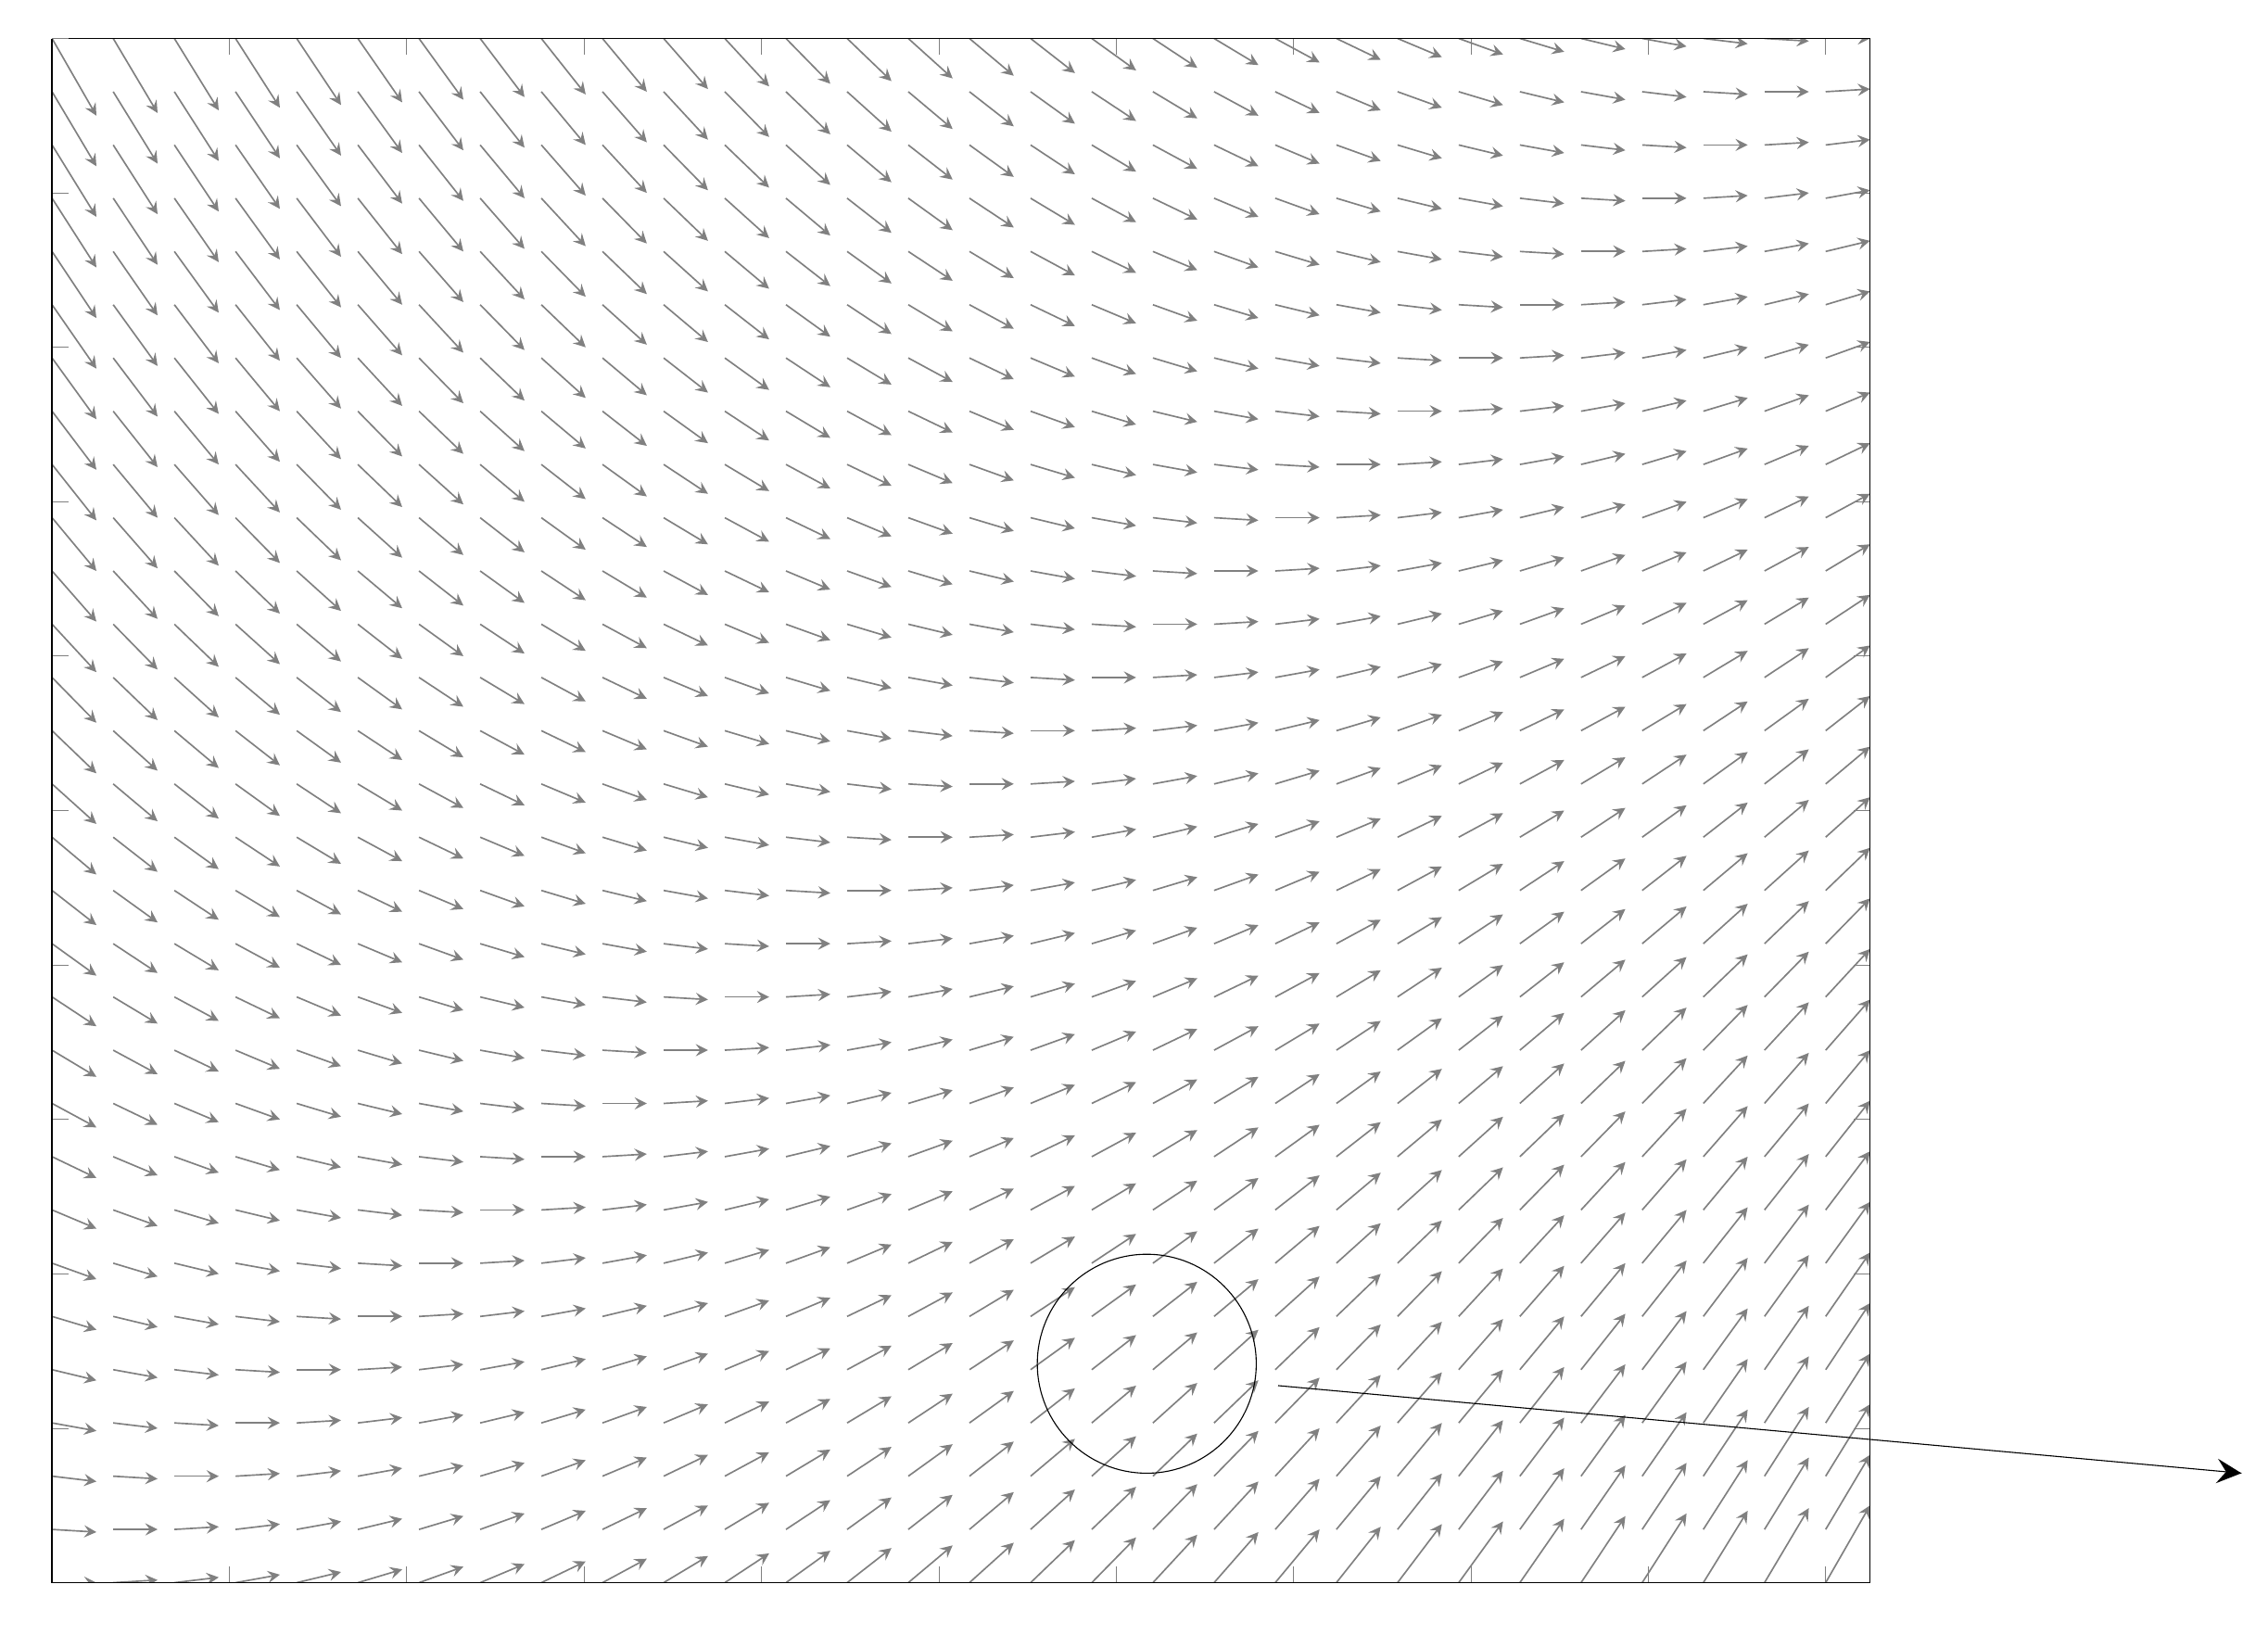
\begin{tikzpicture}[xscale=1.5,yscale=1.5]
\begin{axis}[width=1.5\textwidth,domain=-1:1, view={0}{90}, xtick={}, xticklabels={}, ytick={}, yticklabels={}]
\addplot3[gray, quiver={u={1}, v={(x-y)}, scale arrows=0.05}, -stealth,samples=30] {x};
\end{axis}
\draw (10,2) circle (1cm);
\draw[decoration={markings,mark=at position 1 with {\arrow[scale=3,>=stealth]{>}}},postaction={decorate}] (11.2,1.8) -- (20,1);
\end{tikzpicture}

\hskip-20pt
\begin{honeycomb}
\honey{2}{1}
\end{honeycomb}


\end{document}
